\documentclass[10pt,journal]{IEEETran}
\usepackage[utf8]{inputenc}
\usepackage{graphicx}
\usepackage{hyperref}
\usepackage{tikz}
\usepackage{pgfplots}

\title{Identification d'un utilisateur par la frappe au clavier en l'absence de données d'imposteurs}
\author{Rémi Bourgeon, Franciszek Dobrowolski, Rodolphe Houdas, Timothé Jouglet}
\date{}

\begin{document}

\maketitle

\begin{abstract}
  Dans ce document, nous nous intéressons à la création et la mise en place d'un système d'authentification par la frappe au clavier. Afin de correspondre aux conditions d'utilisation réelles d'un ordinateur, ce modèle sera entraîné sans l'aide de données d'imposteurs.
\end{abstract}

\section{Introduction}
\section{État de l'art}

La recherche en dynamique de frappe au clavier n'est pas récente\cite{wood1977}. En effet, l'idée s'est développée dès l'émergence de systèmes d'exploitation partagés entre plusieurs utilisateurs (UNIX dans les années 1970). L'authentification par nom d'utilisateur et mot de passe est apparue très rapidement comme limitée pour la protection de l'accès aux ressources informatiques, d'où la recherche de nouvelles solutions.

Cependant, après plus de quarante ans de recherche elle est encore loin d'être largement répandue alors que les capteurs d'empreinte digitales sont maintenant monnaie courante sur les \textit{smartphones} et les ordinateurs d'aujourd'hui. Et c'est bien malgré les attraits dont cette technique dispose \textit{a priori} : le faible coût d'acquisition et de traitement des données devrait l'avantager face à toute méthode nécessitant du matériel supplémentaire.

Outre des problèmes de propriété intellectuelle relevés par Peacock \textit{et al.} \cite{peacock2004}, la recherche en dynamique de frappe doit relever de nombreux défis. La qualité de la donnée et le bruit qui peut s'y trouver peuvent fortement influencer les performances du système. Il est donc difficile de développer une solution robuste quand elle à ce point sensible aux biais de la donnée d'entrée. Et dans un contexte où les standards imposent des taux de fiabilité très importants \cite{killourhy2009}, on peut comprendre que la recherche peine à proposer des méthodologies reproductibles pour obtenir des systèmes performants en toute situation.

Il s'avère que le milieu de la recherche en \textit{keystroke dynamics} fait face à un problème de taille, à savoir l'accès à la donnée. Si des travaux ont tenté de normaliser cet aspect de la recherche avec des bases de données publiques de taille respectable \cite{giotGREYC,killourhy2009}, on reste encore loin de jeux de données qui permettraient de s'approcher des situations réelles de certaines applications Web gérant des millions d'utilisateurs.

Néanmoins une autre utilisation que le web nous a parue sous-exploitée. En effet,la dynamique de frappe au clavier \textbf{statique} est largement convoquée dans la littérature existante pour l'identification de \textbf{multiples utilisateurs partageant un secret commun}, tandis que la dynamique de frappe au clavier \textbf{dynamique} est utilisée pour contrôler périodiquement l'authenticité de l'utilisateur du clavier\cite{gunetti2005} (et cette branche est beaucoup plus complexe et moins explorée). Ces deux disciplines sont limitées par le peu de données disponibles pour affiner la recherche.

En revanche, il nous a paru intéressant de se repositionner dans un contexte où la rareté des données est \textbf{non négociable} : dans le cadre d'une \textbf{authentification à deux facteurs} sur une machine personnelle. Dans ce cas précis, la machine ne dispose de toute façons pas de plus de données que celles fournies par son utilisateur. De plus il est inenvisageable d'obtenir des données d'imposteurs pour affiner un modèle en le confrontant à des exemples de données "négatives".

Nous avons donc voulu partir dans la direction de la détection d'imposteur sans disposer de données en grande quantité, ni de données d'imposteurs. Nous nous sommes alors orientés vers les algorithmes de \textit{novelty detection}, et notamment les SVM (\textit{single vector machine}).

La méthode utilisée est largement inspirée par l'article de Chang et Eude\cite{doi:10.1111/coin.12122}.
Dans la section \ref{modele} on utilise une méthodologie de constitution et de validation du modèle de données qui doit beaucoup à cette publication, tout en étant adaptée à un contexte opérationnel différent.


\section{Constitution du modèle}

Notre problèmatique est centrée autour de la constitution d'un système d'authentification en l'absence de données d'imposteurs.

À l'aide de la base de données du GREYC, on peut tracer le positionnement des mesures pour deux utilisateurs distinctssur trois dimensions (voir la figure~\ref{3d}). On peut noter que même dans un nombre faible de dimensions, il semble possible de séparer les mesures en deux groupes distincts représentant chacun un utilisateur. S'il est possible de grouper les données de deux utilisateurs distincts, il est donc possible de définir une frontière de décision qui permet de définir si une nouvelle mesure fait partie ou non d'un groupe donné. On appelle ceci un algorithme de \textit{novelty detection}.

\begin{figure}[b]
    \centering
    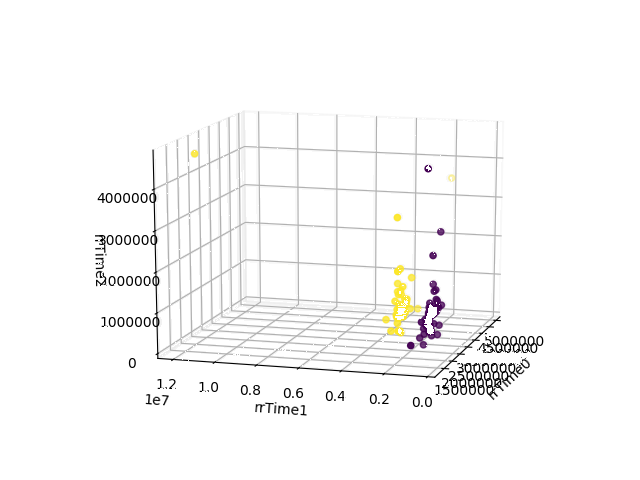
\includegraphics[width=\linewidth]{res/3d.png}
    \caption{Affichage des mesures de l'utilisateur 1 et de l'utilisateur 2 de la base GREYC en fonction des valeurs \textit{rrTime0}, \textit{rrTime1}, \textit{rrTime2}}
    \label{3d}
\end{figure}

Le principal algorithme de \textit{novelty detection} présent dans la librairie \textit{scikit-learn} est l'algorithme de \textit{One-Class SVM}.

Notre travail tente de produire un modèle biométrique basé sur cet algorithme en suivant la méthodologie résumée dans la figure~\ref{ocsvm}, qui récapitule le processus de traitement des données, de constitution du modèle, et d'évaluation de ce même modèle.

\subsection{Pré-traitement des données}

Les données nécessitent d'abord un pré-traitement. Selon la publication \textit{A Practical Guide to Support Vector Classification \cite{svmpractical}}, les données doivent être mises à l'échelle $[0, 1]$ ou $[-1, 1]$. Notre choix s'est porté sur l'échelle $[0, 1]$, qui mettait en évidence de meilleurs résultats lors de l'évaluation des tests préliminaires.

\label{modele}
\subsection{Entraînement du modèle}

L'entraînement du modèle se fait uniquement sur les données utilisateur, c'est-à-dire des données uniquement \textbf{positives}, le jeu de données ne comportant pas d'exemple de données d'imposteurs. Comme pour nombre de modèles d'apprentissage machine, on divise les données en deux lots :

\begin{itemize}
    \item Un lot de données d'entraînement
    \item Un lot de données d'évaluation
\end{itemize}

D'une manière génèrale, il est recommandé d'assigner $4/5$ des données à l'entraînement et $1/5$ des données à l'évaluation. Cette répartition est faite automatiquement lors de la recherche des meilleurs paramètres à l'aide d'un algorithme de \textit{k-fold} : l'entraînement d'un modèle est fait $k$ fois, avec $k$ séparation des données différentes, de manière à trouver les meilleurs coefficients.

Le lot de données d'évaluation est utilisée pour optimiser les paramètres du modèles. Habituellement, cette optimisation se fait à l'aide d'une \textit{recherche par grille de paramètres}, en recherchant les paramètres qui permettent d'obtenir la meilleure précision. Or, dans le cas d'un modèle entraîné sans données d'imposteurs, il n'est pas possible d'obtenir une évaluation de la précision fiable. Il faut donc utiliser une autre mesure pour l'évaluation du modèle : le \textit{rappel}.

Le rappel est "la proportion des items pertinents proposés parmi l'ensemble des items pertinents". Autrement dit, il s'agit de l'ensemble des données détectées comme étant des données utilisateurs sur le nombre effectifs de données utilisateurs. Cette définition n'implique pas la présence de données imposteurs et convient donc à l'évaluation de notre modèle pour la recherche des meilleurs paramètres. Nous chercherons alors à obtenir un rappel qui tend vers 1.

\subsection{Évaluation du modèle}

Une fois le modèle entraîné, on peut l'évaluer avec des données d'imposteurs. Il faut noter ici que cette phase d'évaluation ne sera pas possible lors de l'implémentation d'un logiciel d'authentification par la dynamique de frappe au clavier, en l'absence de données d'imposteurs. Nous l'utilisons ici pour évaluer notre méthode d'entraînement du modèle.

Pour l'évaluation, on utilise toutes les données à notre disposition. Les données utilisateurs seront d'abords divisées en deux lots (un d'entraînement et un d'évaluation). Les données d'entraînement sont passées au module d'entraînement. Le modèle résultant est alors évalué à l'aide des données d'évaluation. On s'intéresse ici au \textit{f-score}, qui est une métrique équilibrant les notions de \textbf{rappel} et de \textbf{précision} pour produire un score significatif.

\begin{figure}[]
    \centering
    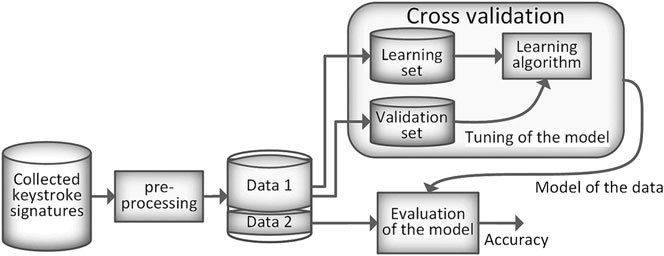
\includegraphics[width=\linewidth]{res/ocsvm.png}
    \caption{Chaîne d'entraînement et d'évaluation d'une One-Class SVM selon Thierry Eude et Chuan Chang\cite{doi:10.1111/coin.12122}}
    \label{ocsvm}
\end{figure}

\section{Capture des données}
\section{Sécurité des données}
Un point central des systèmes d'authentifications, qu'elle qui soit, reste la sécurité.
Le but est de pérenniser les données et dans notre cas le modèle de données. Il est donc impératif de prendre les mesures nécessaires afin de rendre impossible, la falsification du modèle biométrique.

\subsection{Critères de sécurités}
Afin de rendre le modèle le plus sur possible, il est nécessaire d'appliquer des critères précis concernant le modèle et le module d'évaluation.

En premier lieu, il faut s'assurer que le module d'évaluation conserve le même temps de traitement, pour tout type de données et quelque soit son exactitude. La mise en place d'un temps de traitement constant permet d'éviter l'exploitation de cette information par un faussaire, en empêchant de montrer les signes d'un mot de passe erroné.
La solution à cette problématique est la mise en place d'une exécution des tâches de manière asynchrones : toute fonction est exécutée sans attendre la fin de l'étape précédente.

Dans la mesure ou le système biométrique ne soit pas stocker de données d'imposteurs, il est nécessaire que un attaquant ne puisse accéder à d'autres échantillons susceptible de permettre l'accès au modèle.
Afin d'empêcher toute falsification, les échantillons ayant servi à l'entrainement du modèle, ne sont pas stockés. Il en est également de même pour les caractères tapés lors des entrainements et les authentifications.
Dans le cadre de l'algorithme utilisé, ces entités sont déjà prises en compte et ne sont pas garder en mémoire.

\subsection{Chiffrement de la donnée}
Le problème d'utiliser un modèle de Machine Learning correspondant à des profils est qu'il permet d'ouvrir une surface d'attaque à tout faussaire.
Un attaquant qui récupérerait la modèle, pourrait repartir de cette signature, afin d'en générer un autre. De cette faiblesse, il serait donc possible d'outrepasser l'authentification, avec un modèle bien entrainé.
Il est donc vitale de chiffrer les données afin de remédier à cette faille.

Le choix a donc été orienté sur un modèle de chiffrement AES256. Les fonctions de chiffrements et de déchiffrements sont symétriques (utilisation d'une clé) mais reste suffisamment complexe à exploiter. De plus, le fait de ne pas avoir de communication extérieure au système, ne justifie pas l'utilisation de chiffrement asymétrique.
Ce modèle présente plusieurs avantages en termes de ressources, de temps et de sécurité.
Il s'agit d'abord d'un algorithme difficile à casser de manière brutale. La génération aléatoire de clés de chiffrements et l'utilisation d'octets pures, renforce ce modèle.
Le modèle reste pour autant, facile à inclure au modèle et propose un temps d'exécution rapide, ce qui suit l'idée d'uniformisation du temps de traitement. 
Pour ces raisons, le modèle n'en reste que plus sûr.
\section{resultats}

À partir de la base de données du GREYC, nous avons constitué, pour chaque utilisateur possédant plus de 30 enregistrements, 5 modèles. Le modèle affichant le meilleur rappel lors de la phase de pré-évaluation a été retenu et utilisé lors de la phase d'évaluation du modèle.

La figure~\ref{results} représente les FAR et FRR obtenus sur ces modèles lors de la phase d'évaluation pour chaque profil utilisateur testé.

Sur l'ensemble des modèles, on obtient un FRR moyen d'environ $0.21$ et un FAR moyen d'environ $0.10$.

Nous pouvons par exemple remarquer la précision de certains modèles tel que le modèle créé pour l'utilisateur 37 qui possède un FAR d'environ $0.024$ et un FRR d'environ $0.027$ ou le modèle créé pour l'utilisateur 85 qui possède un FAR égal à $0$ et un FRR d'environ $0.033$.

\pgfplotstableset{col sep=semicolon}

\pgfplotstableread{res/graph_data.csv}
\loadedtable

\begin{figure}
\begin{tikzpicture}
\begin{axis}[xbar=0pt,
    bar width=2pt,
    ylabel=Utilisateur,
    xlabel=Valeur,
    ytick=data,
    yticklabels from table={\loadedtable}{userId},
    height=24cm,
    xmin=0,
    xmax=1,
    ymin=0,
    ymax=98,
    width=\linewidth,
    tick label style={font=\tiny}
]

\addplot table[y=nb, x=FRR] {\loadedtable};
\addlegendentry{FRR}
\addplot table[y=nb, x=FAR] {\loadedtable};
\addlegendentry{FAR}
\end{axis}
\end{tikzpicture}
\caption{FAR et FRR pour chaque modèle obtenu}
\label{results}
\end{figure}
\section{Conclusion}

La méthode suivie pour l'entraînement de la \textit{One-Class SVM} et son utilisation produit des résultats peu satisfaisants sur la base de données GREYC. En pratique, à partir des données que nous avions nous même recueillies et exploitées, nous obtenions des résultats plutôt satisfaisants. L'étude des données du GREYC nous montre qu'il y a un certain manque de finesse dans la capture des données et nous pensons que l'utilisation d'un méthode de capture plus précise permettrait d'améliorer les résultats obtenus précedemment.

\bibliographystyle{plain}
\bibliography{bibliography.bib}

\end{document}
